\section{Volunteered Vessel Information}

%"In short, changing technology and economics are moving map production from a system of unified central production to a local patchwork, and the old radial system of dissemination is being replaced with a complex network."
% -- Goodchild cartography paper, old and captures the change in production that is ongoing.

%\citep{elwood2011researching} includes reference to these same layers, capturing data on "core" data layers independently. Covers much of what Goodchild has discussed in terms of issues with VGI and its current "cutting edge".
Historically, ship data were collected both by governments for internal use, and by private corporations for sale. As elsewhere in the production of geographic facts, a shift is underway which moves emphasis away from top-down collection, and toward volunteered information \citep{goodchild2007citizens,elwood2011researching}. Volunteered information has the potential to change our understanding of the ocean, by providing inexpensive and ubiquitous data.

% Using two kinds of volunteered ship data - needs to be handled in special ways:
% describe VOSclim data:
Ship captains have long taken climate observations alongside known locations \citep{brohan2009marine}.  Building on this history, the Voluntary Observing Ship program (VOS, \citealp{VOSOverview}) collects a dataset spanning over 20 years and covering 10\textendash20\% of commercial traffic within each year. As the intention of VOS is purely to collect open-ocean climate data, many participating ships remain anonymous, making reconstruction of ship movements difficult.  The observations are contained within the International Comprehensive Ocean-Atmosphere Data Set (ICOADS, \citealp{woodruff2010icoads}), and though the data are both spatially- and statistically- biased \citep{Wang2007}, it serves as a useful training dataset on ship movements in the open ocean. Here, I use VOS records from 2003--2011, supplemented with opportunistic observations collected by the vessel tracking site SailWX \citep{SAILWX}. Many vessels report both attributes and locations at regular intervals, filling a gap in open ocean observations.
% TODO: what other data does SailWX also include? YOTREPS? what else? Provide details in appendix.

% describe AIS data
The Automatic Identification System (AIS, \citealp{no20041028,Tetreault2002}) was developed to improve maritime safety by providing mariners local situational awareness (Figure \ref{fig:ais-overview}). By locating the ships via global positioning satellite (GPS), and broadcasting vessel location alongside its attributes (Table \ref{table:ais-broadcast-attributes}) via VHF transceiver, mariners gain real-time vessel traffic, invaluable to prevent ship collisions and groundings, and during rescue operations \citep{Itu-r2010}.  The IMO mandates that all ships $\geq\negthickspace 150$ gross tonnage, and ships bearing passengers, must carry AIS units \citep{solas}. This has led to approximately 200,000 ships being outfitted with AIS equipment, including all licensed tankers, cargo ships, and passenger vessels. AIS uses well-understood VHF radios, broadcasting to about 40 kilometers (km) between ships. Since the system's implementation, land-based users, including ports, maritime professionals, and amateurs, have set up VHF antennae, providing low-cost local ship traffic at a range of up to 100km. Numerous sites, such as MarineTraffic \citep{MarineTraffic} and SailWX, provide real-time feeds by aggregating the records from both land-based antennae and satellites, then sharing them using both web maps and Google Earth. These sites augment their networks by providing incentives to users willing to set up new AIS stations, improving coverage over time.

\begin{figure}[htbp]
  \centering
  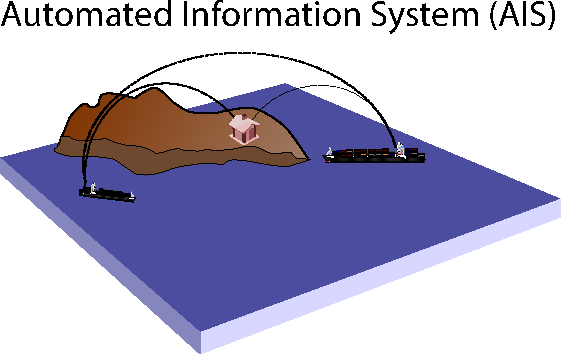
\includegraphics[width=100mm]{figures/towers/drawing-myriad.pdf}
  \caption[Automated Information System diagram]{Automated Information System diagram. Ships communicate to one another via VHF broadcast. The same signals can be captured and stored by land- and satellite- based observers.}
  \label{fig:ais-overview}
\end{figure}

\section{Data Collection}

For this study, fifteen months of AIS observations (November 2010--December 2011) was collected, aggregating records from three major online AIS providers: FleetMon, VesselTracker, and MarineTraffic. All three share Keyhole Markup Language (KML, \citeauthor{KML}) files, intended for use within Google Earth. Examining data availability showed these providers differed in coverage area (Figure \ref{fig:ais-coverage}).  At ten-minute intervals over the study period, I automated downloading these KML files of real-time ship traffic, parsed the files to extract each observation within the KML document, normalized differences between the AIS providers, and finally inserted the results into a spatial database, (\textsf{PostGIS}, \citeauthor{ramsey2005postgis}), an extension that provides support for OGC simple features \citep{OGCSimple} on top of the \textsf{PostgreSQL} \citep{postgresql} object-relational database engine. Over the study period, this resulted in 2.37 billion observations. By comparison, earlier work by \cite{Halpern2008} relied on 2.58 million observations, and that of \cite{Kaluza2010} relied on 490,517 journeys. This manyfold increase requires new methods for analysis, but rewards us with a rich view of shipping. % Oliver: Maybe give a by contrast and emphasize this a bit.  This is much much larger than typical ecological data (the entire eBird dataset is just under 100M observations) and is the key to the methodological challenge that led you to have to develop all sorts of contorted computation tricks.
AIS observations include both ship location and time, and frequently include additional attributes useful for addressing ecological questions (Table \ref{table:ais-broadcast-attributes}).  The VOS/SailWX dataset, consisting of 92.4 million records covering February 1991--September 2011, was provided in a \textsf{MySQL} database dump, which was converted and imported into \textsf{PostgreSQL}. These two sources of observations were then combined with vessel records to provide the validated vessel records used in the analysis (Figure \ref{fig:record-workflow}).

\begin{figure}
  \centering
  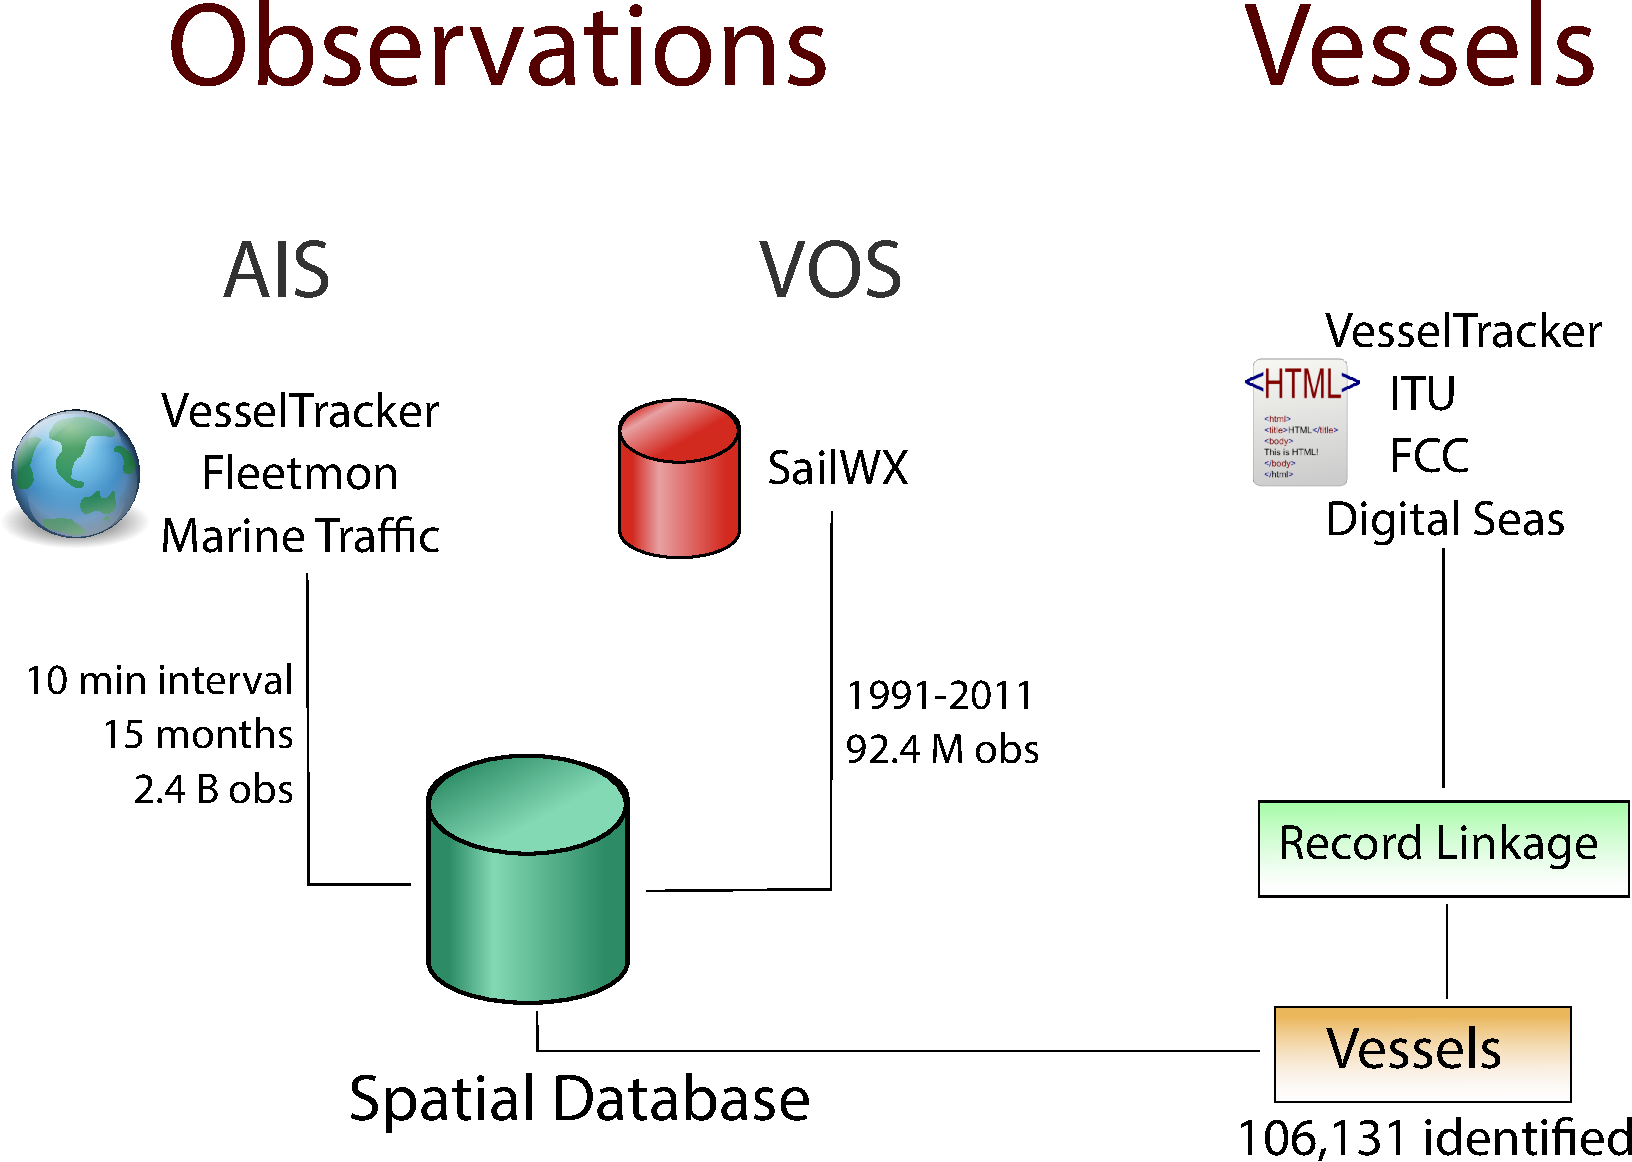
\includegraphics[width=130mm]{figures/record-workflow-myriad.pdf}
  \caption[Data fusion workflow]{Data fusion workflow. Observations from two sources, AIS and VOS, are fused with vessel records to produce tracks of validated vessels.}
  \label{fig:record-workflow}
\end{figure}

To validate the collected ship observations, vessel attribute records and additional ancillary data were identified, as described in the subsequent sections.
% Augmenting these ship observations, ancillary data was identified to provide valid

\subsection{Vessel Attribute Data}
\label{sec:vessel-attribute-data}
Tabular lists of individual ship attributes were collected from both authoritative and crowd-sourced media (Table \ref{table:ships-data-sources}).
\begin{enumerate}
  \item Within the United States, the Federal Communications Commission (FCC) regulates use of the radio spectrum. In order to manage radio licenses, the FCC developed the Consolidated Database System (CDBS), which includes information on all vessels with US-registered radios. 
  \item The International Telecommunications Union (ITU) developed the Maritime mobile Access and Retrieval System (MARS) database to support the maritime community with up-to-date vessel information. Due to their role as a regulating body, participant states are required to provide information at regular intervals. This database is particularly useful as it includes details not available through other public means, such as the vessel owner, and vessel passenger capacity.
  \item DigitalSeas includes volunteered vessel attribute information, collected primarily through corrected AIS observations, but has since gone off-line.
  \item VesselTracker includes ship tracking, reporting and vessel records, alongside real-time AIS position data. Both their vessel data, and their AIS observations were recorded in this study. The dataset shows particular strength for vessels located within European waters. % Vesseltracker has also developed a ship routing network, but does not provide public access to this resource.
\end{enumerate}

\subsection{Land-sea Mask}
\label{sec:land-sea-mask}
  A high resolution land-sea mask, derived from the Shuttle Radar Topography Mission (SRTM) Water Body Data (SWBD, \citealp{slater2006srtm}), classifies the world into either land or sea at a three arcsecond resolution (\textasciitilde{}90m) for much of the world (56$^\circ$ S to 60$^\circ$ N). As a by-product of the SRTM digital terrain project \citep{rabus2003shuttle}, it has the advantage that it was collected over a short period, increasing self-consistency.

For the areas beyond that covered by SRTM, the Global Self-consistent, Hierarchical, High resolution Shoreline Database (GSHHS, \citealp{wessel1996global}) was used, an amalgamation of publicly available shoreline data. GSHHS is lower resolution than SWBD, but the vast majority of ship observations lie within the SRTM study area. The transition between these two layers was manually corrected to make a single, consistent, high-resolution land-sea mask at a three arcsecond (\textasciitilde{}90m) resolution.

\subsection{Supplemental Data}
Port databases were collected, containing coordinates and berth details for ports globally from two sources, the National Geospatial-Intelligence Agency's World Port Index \citep{worldportindex}, and the environmental impact of ports database developed in \cite{Halpern2008}. Approximately 5,000 ports were identified from these two sources.  Qualitative ship movements was also collected, based on historical charts such as a Cold War era CIA chart~(Figure \ref{fig:cia-shipping-map}). The original ship model produced in a previous modeling effort \citep{Halpern2008} was also helpful for comparison.

\section{Validation}
The observations are laden with caveats: because of limitations in the AIS protocol design, there is no direct way of validating a datum \citep{RaymondInPress}, and the VHF transmissions which contain AIS information can be corrupted during transmission. As a result, many terrestrial locations have observations, including a particularly thick band centered around the prime meridian (Figure \ref{fig:ais-obs-nov-2011}). These records are more likely due to corruption of the longitude coordinates than a reverence for Greenwich. In addition to transmission errors are operator errors in any attribute set by the mariner, which is everything other than the location and time provided by the GPS unit. These attributes are frequently either input incorrectly, or not kept up to date for attributes which change over time, such as the destination field. Observations in this dataset are suspect, and here the data are treated as guilty until proven innocent.

While there are inherent errors with the observations, the volume of data and the compiled ancillary datasets both allow us to validate. This validation improves accuracy and minimizes the observations necessary to construct a model representation. Two useful approaches to addressing the validation of large geographic datasets are geographic data mining~\citep{miller2009geographic} and geographic quality checking~\cite{goodchildli2012}. Here, I borrow the framework described in the latter work, and explore three avenues of quality assurance: crowd sourcing, social, and geographic approaches.

\subsection{Quality Assurance}
\paragraph{Crowd-sourcing}
% based (large volume of obs, multiple sources. Crowdsourced ref material)
% TODO EXPAND EXPAND, talk about authority and what it means
While \cite{goodchildli2012} found that crowd-sourcing was generally ineffective for geographic facts, it can function when the domain is limited and the pool of expertise is vast. Crowd-sourcing becomes useful with AIS data when multiple receivers collect the same observation. Cross-referencing these sources provides confirmation, and can be used to measure transmission error.

\paragraph{Social}
Many mariners provide information to online services, and attribute quality from these sources is high. Vessel operators have direct knowledge of a ships' vitals, similar to a neighborhood resident who is likely to have understanding of local geography. The vessel operators then communicate to shipping aggregation sites, who organize a broad collection of vessel data, relying on trusted users to vet updates. These socially filtered records are then used as sources of vessel attribute data (Section \ref{sec:vessel-attribute-data}).

\paragraph{Geographic}
For the error-prone vessel observations, geographic validation is key. Individual observations are point locations with time, and I rely on a handful of tests to provide validation. Each spatio-temporal observation $\langle x, t, z \rangle$ provides point location $x$, time $t$ and multiple vessel attributes $z$.  % Oliver: Just say that each observation <x, t, z> is a combination of point location, x, time, t, and (ship?) attributes, z.
 By cross-referencing the attributes, the joint probability of each attribute can be computed, inferring likelihood on geometry and time from the known traits of a particular vessel.

I impose basic validation on the location by referencing other geographic facts, as is used in the central geographic information system function, the overlay operator. By checking the observations against a composite land-sea mask (Section \ref{sec:land-sea-mask}), I estimate when the provided location is possible. This can be challenging, as many ships travel both by inland waterways such as rivers and canals, so these rules must be careful to define what is traversable, but most vessel classes are restricted to major water bodies and a handful of large canals. Shallow water imposes an additional constraint, depending on ship draft. This can be used to show, for example, the distance oil tankers keep from land masses.

% Oliver: I do not cause a lot of ecological disruption when I go traipsing through downtown, but if I go trampling through the Los Padres, I can cause a lot of harm.  I would say people disproportionately occupy developed areas, yet there is a lot of ecological harm caused by outliers.
For most vessel transportation classes, ships move between ports. In these classes, ships exhibiting patterns inconsistent with port-to-port movement are suspect.  However, there are other fixed locations besides ports which require inclusion, such as ballast water exchange points, like one located 100 nautical miles (nm) offshore of California (Figure \ref{fig:cal-cargo}), and canals, which enable movement between otherwise disconnected locations. Generally, port location is useful: because AIS receiving towers tend to be near ports, the data captures the origin and destination pairs of most vessel journeys. Finally, I require observations have coordinates bounded by the coordinate space, and exclude any beyond the surface of the earth. 

% TODO: expand this, what else do we do?

\section{Data Representations}
% It is necessary to have multiple representations of the data - the data model must flow from the question asked (goodchild, also anything in ebook on GISci?)

%Want to link representation to USE, lack of a single simple view which meets all needs. counterpoint to the 'single metric' perspective. 
% [have note: "link to stats", but now unsure what that means].
Ship observations are contributed by vessels on both a voluntarily and mandated basis, and using geographic quality checking methods produces a validated set of observations. And while individual observations have a simple representation (a location, time, and attributes), effective use requires multiple representations \citep{Goodchild1992} and the spatio-temporal modeling techniques of time geography \citep{miller2008field}.  Because there is no single, optimal representation of data, we produce a set of representations which, when matched to particular uses, can provide insight.  Here, I maintain both discrete object and continuous fields representations (Figure \ref{fig:representation-in-gis}), to address questions about the ecological effects of shipping. While the point representation alone is too simple for understanding shipping's effects, incorporating too much complexity in the representation risks making computation infeasible~\citep{de2007geospatial}.

% The spatial databases' historical focus was on accuracy \citep{goodchild1989accuracy}. This showed the value in retaining raw observations, both by minimizing lossy transformations, and providing multiple models of the same data to retain consistency with reality.

% Some of the effects. link up how specific effects could be monitored by our different representations. Can't just use points to predict phenomena of this nature, but can't incorporate full complexity of reality either; chosen representations are a compromise between those two extremes.

\begin{figure}
  \centering
  \hspace*{-0.25in}
  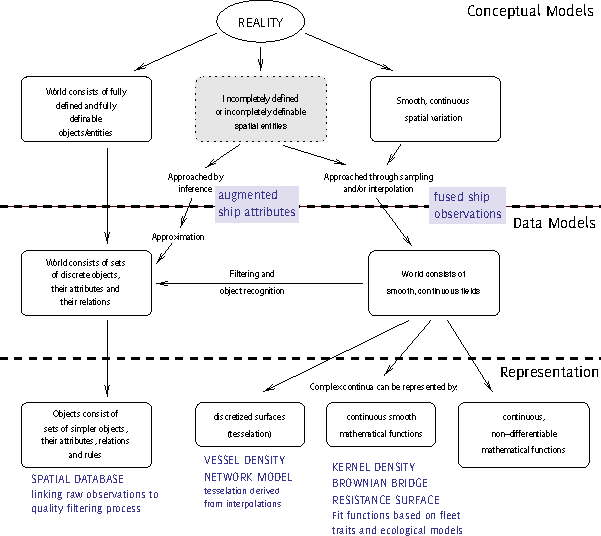
\includegraphics[width=155mm]{figures/representation-in-gis-myriad.pdf}
  \caption[Spatial abstractions]{Spatial abstractions, this work's {\color{DBlue} representations in blue}. Adopted from \cite{Bivand2011}, based on original by \cite{burrough1996geographic}.}
  \label{fig:representation-in-gis}
\end{figure}

% TODO What am I really trying to say? We need to maintain multiple representations. Why? Different questions require insight into different features of the data. PROVIDE EXAMPLES: traits, distribution of ship speeds needed for whale-vessel interactions (ship strikes). Need vessel attributes, movement tracks, engine type, ... for sound. Walk people through this so they can understand it more easily.
One representation developed is speed density (Section \cite{ref:ship-density-estimates}), useful for understanding whale-vessel interactions. Combining vessel type, vessel draft, and vessel length with a derived speed estimate, we can spatially model vessel risk in whale-vessel encounters. Similar combinations of vessel attributes and derived representations are useful for other ecological questions.

\subsection{Ship Types}

% see fleet-size-and-naming.txt for details on the ship validation issues.
% SHIP CLASSES! HOW ARE THEY DEFINED, WHAT ARE THE DIMENSIONS BEING COLLAPSED?
%  a bunch of ways to classify (included in wikipedia article, I also have some notes we defined these by functional groups and their expected ecological differences

An open problem in the maritime community is how to designate ship types. Ships can be classified on a variety of dimensions, including: engine type, hull material, vessel function, and size. Ontologies have been developed to address the problem, but remain incomplete \citep{Vries2009}. Here, I focus on use, and rely on the primary activity the vessel is engaged in. Starting with the classes provided by our AIS and VOS sources, I collapsed them into nine major functional groups: authority, cargo, fishing, high-speed, passenger, pleasure, support, tanker, and ``other'' for vessels which don't map into any of our primary classes. Because the full attributes of each vessel are retained, and frequently includes multiple type labels, it is possible to break this down further for future analyses, but these broad classes served well for classifying distinct movement patterns. A full list of vessel classes is provided in Appendix \ref{table:ship-class-breakdown}.

As AIS is mandatory for cargo, tanker, and passenger ships, making classification of the vessel population in these classes representative. Other classes, such as authority, here represent a limited subset of search and rescue vessels, not naval or police vessels. Fishing vessels are similarly a limited representation, only specific areas which mandate AIS have any observations, so classes such as artisanal fishing aren't present.

\subsection{Ship Identifiers} 

Identifiers, designating which ship a particular vessel is from, also poses a problem. By incorporating information from many different identifiers and focusing on those less fluid, such as IMO number and radio callsign, we increase the chances of valid matches. However, additional attributes such as the Maritime Mobile Service Identity (MMSI), and vessel name remain useful, particularly because they are broadcast alongside each AIS record. Vessel operators may not maintain this information, making it important to cross-validate the attributes to improve match rates.

\subsection{Point Data}

AIS records are sampled at 600 second intervals (10 minutes). For most vessel classes, this sample rate retains the movement patterns, and is a similar rate to that used in studies using aggregation to remove noise, such as \cite{Vries2009}, which uses piecewise aggregate approximation at a 300 second interval to ``strike a good balance between capturing the general movement and ignoring noise''. % XXX NOTE: this is a filtering technique, so it isn't a direct mapping onto the reduced fidelity data we're using.

% TODO: add more details here.

\subsection{Tracks}

Tracks convert discretely sampled time points $\langle x, t \rangle$ into a interpolated continuous phenomena. The uncertainty surrounding the interpolation can be described by a time prism (Figure \ref{fig:time-prism}), which bounds the area based on the maximum velocity of the object at motion. Here, I constrain the track segments to have movement speed above 0.5 Knots (Kt)/hr, below which vessel control is difficult, and speed below 40 Kt/hr, which derived empirically from our ship speed distributions (Figure \ref{fig:vessel-speed-density} and vessel engine characteristics.  I further require that to be considered a track, the above criteria must be met for at least one segment of that vessel's transit. The ships are then constrained to move along the shortest distance on a geoid, or great circles, using GeographicLib \citep{karney2012algorithms}. This information is reused in computing the speed along each segment. % XXX Oliver: Aren't the speed and on-planet requirements applied to all segments of the track anyway?; TOO TECHNICAL?
% some of above pulled from tracks/shipping_tracks_obs_validated.py

\begin{figure}[h!]
  \centering
    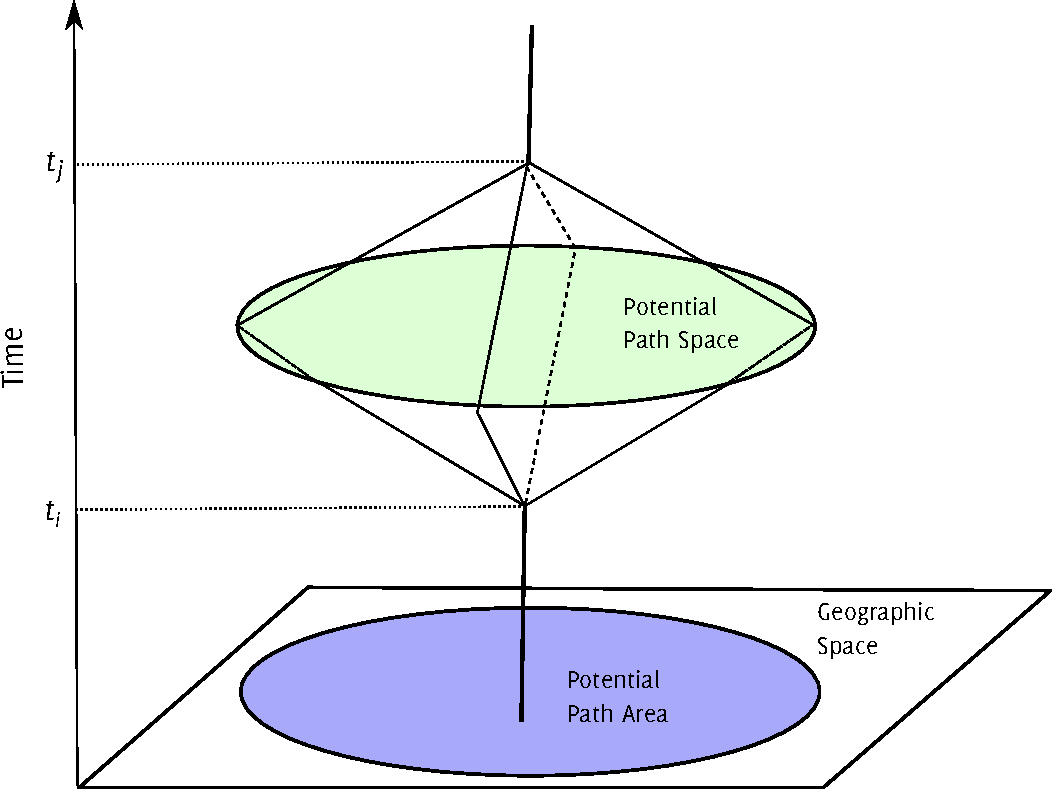
\includegraphics[width=100mm]{figures/time-geography-prism.pdf}
  \caption[A simple space{\textendash}time prism]{A simple space{\textendash}time prism; based on \cite{Wu2002}.}
  \label{fig:time-prism}
\end{figure}

% XXX XXX XXX
% XXX XXX XXX
% XXX XXX XXX
% XXX XXX XXX INTEGRATE THIS to get the multiple representation + time geography story down.
Ship observations are contributed by vessels that submit data on both a voluntarily and mandated basis \citep{VOSClim,Tetreault2002}, affording an opportunity to advance our use of geographic quality checking methods \citep{goodchildli2012} against this volunteered geographic information (VGI, \cite{goodchild2007citizens}). And while individual observations have a simple representation (a location, time, and attributes), effective use requires multiple representations \citep{Goodchild1992} and the spatio-temporal modeling techniques of time geography \citep{miller2008field}.
% XXX XXX XXX

%   \item link to time geography... Hagerstrands conceptual framework... Literature on T-GIS as tracking.
%   \item Goodchild lecture on T-GIS mentioned track interpolation, inferences about activity, track convergence, etc
 % [perhaps drop this for the time being... don't have lit built up on it, unless we can use the anomaly detection stuff]

\subsubsection{Field-based Models}

Initially, kernel density estimation was used to produce field based estimates. However, based on the data volume, it proved more useful to provide models directly from discretized tracks, which are used in the two following datasets.

\paragraph{Ship density by type}

The primary output of this work is a field-based density model of ship movement. This view is useful in a wide variety of contexts, from exercises in marine spatial planning to detecting conflict zones between resource users, and the simple density estimation in \cite{Halpern2008} remains a highly requested product. % XXX provide better examples
% XXX Why this matters: the view most people want to see; counts of X where and when. Useful for MSP, conflict resolution, detecting conflict zones, etc

Each vessel track was rasterized to both an 90 arcsecond grid (\textasciitilde{}5.5km at the equator) and an equal area grid in the Hobo Dyer projection (Figure \ref{fig:eu-cargo-density}). The latter case assures that the density function is computed on grid cells representing the same area for each cell, unlike the geographic grid where area varies by latitude. A vessel is counted only once for each cell it passes through, as the focus here on overall movement patterns, and this criteria helps de-emphasize vessels with limited movement. Each raster vessel track was combined using simple map algebra to produce density maps for both the AIS and VOS data, for each of our vessel classes. % XXX Oliver: A passing cargo ship is comparable to a ferry crisscrossing the same spot continuously every day?  Not that you should do this, but somebody might wonder.

For each cell, the output density $s$ is calculated as the standardized equal-weighted addition between the two inputs:
\begin{equation}
 s = \frac{R_{AIS}}{max(R_{AIS})} + \frac{R_{VOS}}{max(R_{VOS})} 
\end{equation}
% XXX Oliver: Why can't you calculate actual average speed using segment lengths?  Some jerk is going to ask. <- self-fulfilling

\paragraph{Speed density estimations of ships by ship type}
\label{ref:ship-density-estimates}
Ship speed plays a critical role in determining the survivability of collisions for many marine species~\citep{Vanderlaan2009}. Speed also directly relates to the emissions profile of a vessel, and it has been shown that speed reduction alone can reduce 50-80\% of greenhouse gas emissions~\citep{lack2011impact}. Conversely, decreased speeds require more vessels to ship the same volume of goods or passengers, though companies such as Maersk are mitigating this by moving to significantly larger capacity container ships. 

Average speed per cell was calculated as sum speed over all observations $R_{AIS} \cup R_{VOS} = n$, and dividing it by the total number of observations, but only for those locations where a sufficient density $s$ is present: 

\begin{equation}
 \bar{s} = \left\{
   \begin{array}{l l}
    \frac{\sum\limits_{i=0}^n s}{x} & \quad \text{$s \ge 10$}\\
    0 & \quad \text {$s < 10$}
   \end{array}\right.
\end{equation}

% CLARIFY: what are the other effects of speed? anomaly detection?

% calculated the ship average speed over the journey, used that as 'speed value' [pretty bogus, but was quick and I couldn't get the M values in OGR correctly].

%Some analyses require "factoring out" geography to the extent possible, such as ecological models (Tilman book), Economic, et cetera. Network theory provides a useful basis of analysing geographically explicit data in a mathematical framework which can incorporate some of the geographic constraints while eliding many details necessary in a spatially-explicit model.

% another pp from a position
% This becomes particular important as the tools of spatial thinking extend across disciplinary boundaries, both in the social and physical sciences (Goodchild and Janelle, 2010; Tilman and Kareiva, 1997). Other domains, such as ecology and economics, are coming to terms with the fact that their historical approaches to keeping simple models (and by extension, limiting model scope to their domain) ignores important spatial context which naturally arises at the unit of analysis (Tilman and Kareiva, 1997; Krugman, 1991).

\section{Record Linkage}

By combining authoritative data from a variety of sources (Table \ref{table:ships-data-sources}), we can reconcile our observations, greatly improving the quality of resulting ship movement models. Though we do include two authoritative datasets, the sources are inconsistent, and require an initial step of cross-linking records. This approach was initially developed with medical records, and more recently developed as the record linkage field in computer science~\citep{Christen2012}.

% table describing sources
% SOURCES: ship-id-model.txt
%          ship-id-model/linkages.txt
\begin{table}
  \caption[Ship data sources]{Ship data sources.}
  \tabcolsep=0.11cm
  \renewcommand{\arraystretch}{0.7}
  \begin{tabular}{rrrrl}
    \hline
    Source & Code & Records & Linked & Attributes \\
    \hline
     Digital Seas & DS & 212166 & 68002 & name, IMO, MMSI, callsign, type, \\
                  &    &        &       &  width, length \\
      FCC\textsuperscript{1} ULS\textsuperscript{2} & FCC & 319964 & 24531 & name, MMSI, callsign, class,\\ 
                                                    &     &        &       & gross tonnage, length \\
      ITU\textsuperscript{3} MARS\textsuperscript{4} & ITU & 372183 & 75928 & name, IMO, MMSI, callsign, \\ 
                                                     &     &        &       & class, owner, gross tonnage \\ 
     VesselTracker & VT & 126534 & 83372 & name, IMO, MMSI, callsign,\\
                   &    &        &       & class, length
  \end{tabular}
  \\
  \\
  \footnotesize{1. Federal Communications Commission; 2. Universal Licensing System;  3. International Telecommunication Union; 4. Maritime mobile Access and Retrieval System}
  \label{table:ships-data-sources}
\end{table}

I built a probabilistic model which evaluated all possible pairwise combinations between source records. By using the methodology of record linkage, a set of rules was developed to map records between the six possible source pairs. Each pair was evaluated for common, consistent attributes, and compared against these columns. The software package used, (FRIL, \citealp{Jurczyk2008fril}), provides an Expectation Maximization algorithm to iteratively optimize the column weighting, but due to the large number of records, this proved ineffective. Instead, samples were examined, and the criteria were set by tuning both the weightings and acceptance levels to match a training dataset of valid linkages (Table \ref{table:ships-record-linkage-methods}). 

For most attributes, either the equal fields (both values are the same) or the Jaro-Winkler distance metric were used. Jaro-Winkler has useful properties for this data: it is effective on both numeric and textual data, and is particularly good in picking up the kinds of errors inherent in user provided data sources such as those used in this study. A study of string comparison metrics found it to be both efficient, and effective, with a high match rate on diverse data~\citep{Cohen2003}. The equations used in the Jaro-Winker distance are described in Appendix \ref{sec:record-linkage-appendix}.

Once each combination between two sources was finished running in FRIL, a second rule-based method was developed to capture valid pairings initially missed. If vessels had equality in any two attributes of the set \{MMSI, callsign, name\}.  If callsign and vessel length matched, or if the IMO number provided was a valid seven digit number, then the pair was marked as linked. This was tested against a number of pairs manually, and successfully caught many of the initially missing yet valid linkages.

\subsection{Linkage Validation}

Detecting errors in this data are particularly problematic, as the records are highly correlated by nature -- often, IMO number, callsign and name differ by only one character for two ships in the same fleet. We want to keep these kinds of vessels separate, while simultaneously finding small differences due to entry error, which proved difficult. I developed a validation score to remove over-aggressive links between the data, and allow us a second quality check which is tunable to threshold the data, depending on the kinds of error we are willing to accept.

To start with, I evaluated the invalid joins present in the data, and the specific traits that were common across the sample. These included:
\begin{enumerate}[noitemsep]
 \item >6 linked records
 \item >1 radio callsign
 \item >1 MMSI
 \item clear name mismatches
 \item vessel assigned to multiple incompatible classes
\end{enumerate}

Based on this, a set of rules was developed to assign a validation score and probable vessel class based on the inputs.  Again Jaro-Winkler was used to compare attribute matches for both ship name and radio callsign, with $1 - d_w$ being added to the score. For attributes that had a single value, the attribute score was increased by one, otherwise vessels which had more than two MMSIs or five linked records had one point removed from their score. Finally, if a ship was identified as being in multiple incompatible classes, one point was subtracted for each additional class. Our final scores for all vessels are shown in (Figure \ref{fig:validation-score-hist}).

\begin{figure}[h!]
  \centering
    \includegraphics[width=150mm]{figures/validation-scores-hist.pdf}
  \caption[Linkage validation scores]{Linkage validation scores, bin width=0.3}
  \label{fig:validation-score-hist}
\end{figure}

Only those vessels with validation scores exceeding zero were used in the movement models, and the validation class provides our chosen class for each validated vessel. Finally, though all these steps give us good self-consistency, I wanted to test against even better sources.  % TODO: perform data validation on these observations with Equasis. Sample a handful of records from each class, then perform the validation.
While some of our input datasets are authoritative, the best available data remains commercial. A 1\% sample of the records were compared to those provided in Equasis \citep{Equasis2011}, which includes validated records from the commercial fleet. This showed that, after cross-linking, the validation score showed good correspondence with true vessels.

% XXX XXX XXX
% XXX XXX XXX

\subsection{Uncertainty and Limitations}

- at a minimum, include our "obs per area" figure to show what kind of density we have, what \% of major world ports is sampled.
- ports: of large ports in WPI, 112/155 (72.3\%) had 100 or more unique vessels, and 187/357 (52.4\%) of medium ports, we have AIS for much, but not all of the important near shore areas.

mention the difficiencies of some areas (why are we routing some data through land masses?)

Only have single average vessel speed
Don't have detailed attributes for each segment.
